\documentclass[tikz,border=2pt]{standalone}
\usepackage{amsmath,amssymb}
\usepackage{tikz}
\usetikzlibrary{arrows.meta}

\begin{document}
% Slack variables at the interior point (20,20): s_1 = 100 - 2*20 - 20 = 40 unused finishing
% hours, s_2 = 40, s_3 = 20; on a constraint line the corresponding slack is zero.
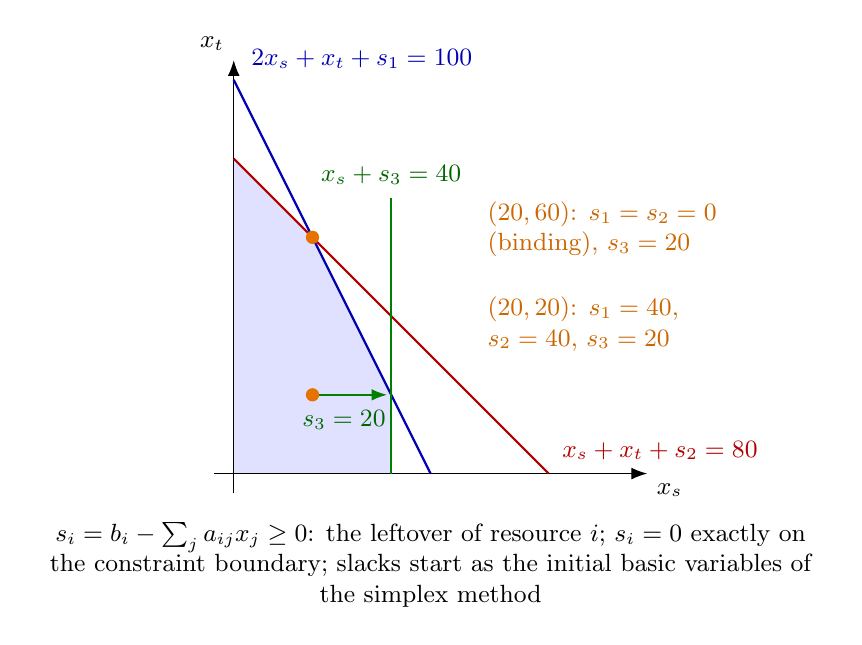
\begin{tikzpicture}[x=0.05cm, y=0.05cm, every node/.style={font=\small}, >={Latex[length=2mm]}]
	\fill[blue!12] (0,0) -- (40,0) -- (40,20) -- (20,60) -- (0,80) -- cycle;
	\draw[->] (-5,0) -- (105,0) node[below right] {$x_s$};
	\draw[->] (0,-5) -- (0,105) node[above left] {$x_t$};
	\draw[blue!70!black, thick] (50,0) -- (0,100);
	\draw[red!70!black, thick] (80,0) -- (0,80);
	\draw[green!50!black, thick] (40,0) -- (40,70);
	\node[blue!70!black, font=\small, anchor=south west] at (2,100.5) {$2x_s+x_t+s_1=100$};
	\node[red!70!black, font=\small, anchor=south west] at (81,1) {$x_s+x_t+s_2=80$};
	\node[green!40!black, font=\small, anchor=south] at (40,71) {$x_s+s_3=40$};
	\draw[->, green!50!black, thick] (20,20) -- (39,20);
	\node[green!40!black, font=\small, anchor=north] at (28,18.5) {$s_3=20$};
	\fill[orange!90!black] (20,20) circle (2.4pt);
	\fill[orange!90!black] (20,60) circle (2.4pt);
	\node[orange!80!black, font=\small, anchor=west, align=left] at (62,62) {$(20,60)$: $s_1=s_2=0$\\ (binding), $s_3=20$};
	\node[orange!80!black, font=\small, anchor=west, align=left] at (62,38) {$(20,20)$: $s_1=40$,\\ $s_2=40$, $s_3=20$};
	\node[anchor=north, align=flush center, text width=10cm] at (50,-10) {$s_i=b_i-\sum_ja_{ij}x_j\ge0$: the leftover of resource $i$; $s_i=0$ exactly on the constraint boundary; slacks start as the initial basic variables of the simplex method};
\end{tikzpicture}
\end{document}
